\documentclass[11pt]{beamer}
\usetheme{default} 

\setbeamertemplate{navigation symbols}{} %gets rid of navigation symbols
\setbeamertemplate{footline}{} %gets rid of bottom navigation bars
\setbeamertemplate{footline}[page number]{} %use this for page numbers

\setbeamertemplate{footline}{%
  \raisebox{5pt}{\makebox[\paperwidth]{\hfill\makebox[10pt]{\scriptsize\insertframenumber~~}}}}

\setbeamertemplate{itemize items}[circle] %round bullet points
\setlength\parskip{10pt} % white space between paragraphs

\usepackage{wrapfig}
\usepackage{subfig}
\usepackage{setspace}
\usepackage{enumerate}
\usepackage{graphicx}
\usepackage{amsmath}
\usepackage{amsfonts}
\usepackage{amssymb}
\usepackage{amsthm}
\usepackage[UKenglish]{isodate}
\usepackage{tikz}
\usepackage{pgfplots}
\usepackage{natbib}
\def\checkmark{\tikz\fill[scale=0.4](0,.35) -- (.25,0) -- (1,.7) -- (.25,.15) -- cycle;} 

% allow drawing arrows
\usetikzlibrary{arrows}
\tikzstyle{arrow}=[draw, -latex] 

% skips
\setlength{\abovecaptionskip}{15pt plus 3pt minus 2pt}
\setlength{\belowcaptionskip}{5pt plus 3pt minus 2pt}
% bracketing shortcuts
\newcommand{\paren}[1]{\left(#1\right)}
\newcommand{\sqbracket}[1]{\left[#1\right]}
\newcommand{\cbracket}[1]{\left\{#1\right\}}
\newcommand{\abs}[1]{\left\lvert#1\right\rvert}
\newcommand{\norm}[1]{\left\lVert#1\right\rVert}
% set up the argmin operator, argmax
\DeclareMathOperator*{\argmin}{arg\,min}
\DeclareMathOperator*{\argmax}{arg\,max}

\newcommand{\myframe}[1]{\begin{frame} \frametitle{#1}}
% New itemize environment, with spaces
\newenvironment{spaceitemize}
{ \begin{itemize}
    \setlength{\itemsep}{10pt}
    \setlength{\parskip}{0pt}
    \setlength{\parsep}{0pt}     }
{ \end{itemize}                  } 

% the preamble
\title{Day 2, Session 1: Graphs}
\author{Brian D. Williamson}
\institute{EPI/BIOST Bootcamp 2017}
\date{25 September 2017}

% Start the document
\begin{document}
% The title page
\begin{frame}
\titlepage
\end{frame}

\section{Types of graphs}
\myframe{Graphs}
Why do we use graphs?
\begin{itemize}
\item \textcolor{blue}{Describe relationships} in the data
\item[]
\item Visualize functions
\end{itemize}

Graphs are very useful in exploratory analyses, or for description. Often a graph (or multiple graphs) provide \textcolor{blue}{visual evidence that supports a statistical analysis}.

\end{frame}

\myframe{Example data analysis: FEV \small (from Scott Emerson, MD PhD)}
Based on numerous studies, we believe that smoking tends to impair lung function. Much of the data to support this claim arises from studies of long-term adult smokers. A natural question is: can deleterious effects of smoking be detected in children who smoke?
\begin{spaceitemize}
\item Data on 654 children seen during routine check-up at pediatric clinic
\item Outcome: forced expiratory volume (FEV)
\begin{itemize}
\item measures how much air you can blow out of your lungs in a short period of time
\item higher FEV typically associated with better respiratory function
\end{itemize}
\item Predictor of interest: smoking status
\item Other variables: sex, age, height
\end{spaceitemize}
\end{frame}

\myframe{Common types of graphs in data analysis}
\vspace{-1em}
\begin{figure}
\centering
\subfloat[Histogram]{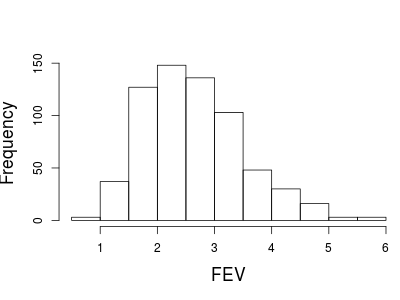
\includegraphics[width=.4\textwidth]{figs/day_2_graphs_hist_example.png}}
\hspace{1cm}
\subfloat[Boxplot]{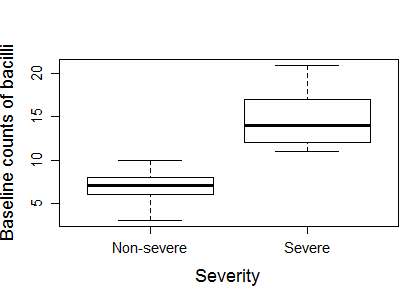
\includegraphics[width=.4\textwidth]{figs/day_2_graphs_bplot_example.png}}

\subfloat[Scatterplot]{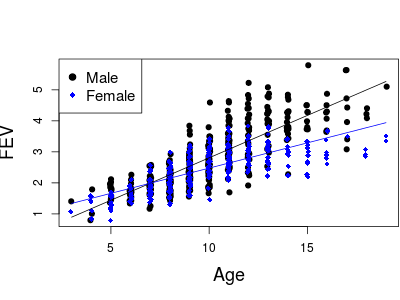
\includegraphics[width=.4\textwidth]{figs/day_2_graphs_scatplot_example.png}}
\end{figure}
\end{frame}

\myframe{What do graphs tell us?}
\begin{itemize}
\item Histograms: summaries of one-dimensional distributions
\begin{itemize}
\item Counts or frequencies of each occurrence
\end{itemize}
\item[]
\item Boxplots: summaries of two-dimensional distributions
\begin{itemize}
\item measures of center (typically median)
\item[]
\item measures of spread (typically inter-quartile range)
\end{itemize}
\item[]
\item Scatterplots: summaries of two-dimensional distributions
\begin{itemize}
\item Can visualize the whole data
\item[]
\item Trends in two or more dimensions by using different colors/shapes for strata
\end{itemize}
\end{itemize}
\end{frame}

\section{Linear trends}
\myframe{Linear trends}
\begin{spaceitemize}
\item A common way to describe data---determine if the trend is increasing or decreasing
\begin{itemize}
\item Example: test scores tend to increase with time spent studying
\end{itemize} 
\item Lines are easy to compute
\begin{itemize}
\item Only need a point and a slope
\item[]
\item Two common forms of linear equations
\end{itemize}
\end{spaceitemize}
\end{frame}

\myframe{Slope-intercept form}
\begin{itemize}
\item $y = mx + b$
\item[]
\item Slope: $m$
\begin{itemize}
\item Rate of change, i.e., how does $y$ change with each one unit change in $x$?
\item[]
\item Example: speed, the distance traveled with each unit change in time
\end{itemize}
\item[]
\item Intercept: $b$
\begin{itemize}
\item The point where the line crosses the $y-$axis
\end{itemize}
\end{itemize}
\end{frame}

\myframe{Example: FEV}
Fitting a trend line to a scatter plot of the FEV data helps us understand the association between age and FEV. If we use the \emph{least squares} criterion to fit this line (you'll learn more about this when you cover linear regression), we obtain the plot below:

{\centering
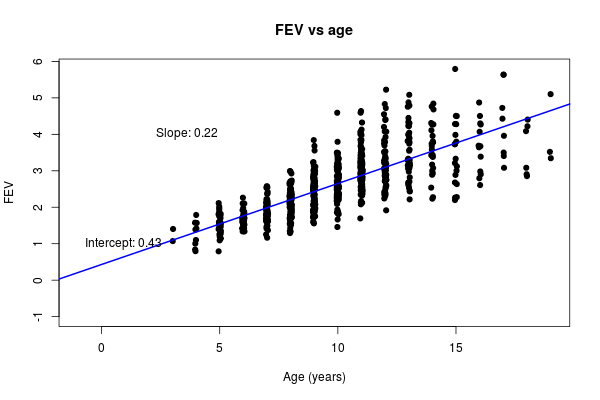
\includegraphics[width = 0.7\textwidth]{figs/fevline.png}
}

\end{frame}

\myframe{Example: FEV}
The intercept, 0.43, is interpreted as the \textcolor{red}{mean FEV for children at age zero} (\textcolor{purple}{does this make sense?}). The slope, 0.22, is interpreted as the \textcolor{blue}{mean increase in FEV for each one year increase in age}, where older children tend to have higher mean FEV.

How do the slope and intercept together determine a line? What happens to the interpretation of our regression coefficients (which is what the slope and intercept are in this example) if either one of these values is different?
\end{frame}

\begin{frame}
\frametitle{Slope-intercept form: determining a line}
\centering
\begin{tikzpicture}
\begin{axis}[
    axis lines=middle,
    xmin=-15, xmax=15,
    ymin=-15, ymax=15,
    xtick=\empty, ytick=\empty,
    xlabel=$x$, ylabel=$y$
]
\addplot[mark=*] coordinates {(0,0.43)} node[pin=150:{\small Intercept $(0,0.43)$}]{} ;
\end{axis}
\end{tikzpicture}
\end{frame}

\begin{frame}
\frametitle{Slope-intercept form: determining a line}
\centering
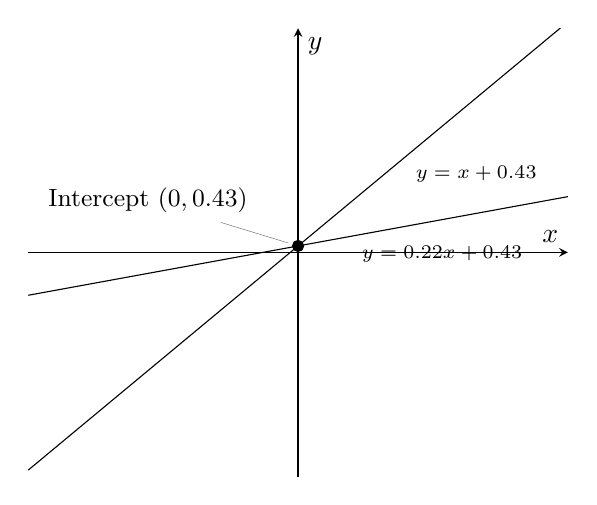
\begin{tikzpicture}
\begin{axis}[
    axis lines=middle,
    xmin=-15, xmax=15,
    ymin=-15, ymax=15,
    xtick=\empty, ytick=\empty,
    xlabel=$x$, ylabel=$y$
]
\addplot[mark=*] coordinates {(0,0.43)} node[pin=150:{\small Intercept $(0,0.43)$}]{} ;
\addplot [domain=-15:15, samples=2] {0.22*x+0.43} node [pos=.6, below right] {\scriptsize $y = 0.22x + 0.43$} ;
\addplot [domain=-15:15, samples=2] {1*x+0.43} node [pos=.7, below right] {\scriptsize $y = x + 0.43$};
\end{axis}
\end{tikzpicture}

What is the difference between the two slopes? How does this affect our understanding of the association between age and FEV?
\end{frame}


\myframe{Point-slope form}
\begin{itemize}
\item $y - y_1 = m(x - x_1)$
\item[]
\item Point: $(x_1, y_1)$
\begin{itemize}
\item A point on the line (can be any point! Even the intercept!)
\end{itemize}
\item[]
\item Slope: $m$
\begin{itemize}
\item Same as in slope-intercept form!
\end{itemize}
\item[]
\item Example: $y - 0.43 = 0.22(x - 0)$ is the same as $y = 0.22x + 0.43$ in slope-intercept form!
\end{itemize}
\end{frame}

\myframe{Exercise: slopes and intercepts}
Consider data examining inflammatory biomarkers and mortality. We are interested in the association between the the biomarker fibrinogen (related to inflammation) and prior history of cardiovascular disease (CVD). These data are described \href{https://www.emersonstatistics.com/datasets/inflamm.doc}{here}. Your collaborator ran a linear regression and obtained the following equation (using the estimated regression coefficients), where $y$ denotes fibrinogen (ranges from 109 mg/dl to 872 mg/dl) and $x$ denotes presence/absence of prior CVD (0/1): $y = 14.89x + 319.57$.
\begin{enumerate}
\item What is the slope of the line $y = 14.89x + 319.57$?
\item[]
\item What is the $y-$intercept of the line $y = 14.89x + 319.57$?
\item[]
\item Does fibrinogen tend to increase or decrease with the presence of prior CVD compared to the absence of prior CVD?
\item[]
\item What is the slope of the line $y + 1 = 2(x - 1)$?
\item[]
\item What point did we use to create the line $y + 1 = 2(x - 1)$?
\end{enumerate}
\end{frame}

\myframe{Solution: slopes and intercepts}
\begin{enumerate}
\item The equation is in slope-intercept form, so the slope is 14.89
\item[]
\item The equation is in slope-intercept form, so the intercept is $319.57$
\item[]
\item The slope estimate is positive, so fibrinogen tends to increase with presence of prior CVD
\item[]
\item The equation is in point-slope form, so the slope is 2
\item[]
\item The equation is in point-slope form, so the point is $(1, -1)$
\end{enumerate}
\end{frame}

\myframe{Creating a graph using an equation}
\begin{itemize}
\item Steps:
\begin{enumerate}
\item Draw axes
\item[]
\item Place a point at the $y-$intercept (slope-intercept form) or at the starting point (point-slope form)
\item[]
\item Increase $x$ by one unit, increase $y$ by $m$ units, place a new point
\item[]
\item Draw a line between the old point and the new point!
\end{enumerate}
\end{itemize}
\end{frame}

\myframe{Example: creating a graph using an equation}
\centering
\begin{itemize}
\item Equation $y = 0.22x + 0.43$ (from linear regression of FEV on age, in the FEV data)
\item[]
\item Slope: 0.22, Intercept: $0.43$
\item[]
\item[1.] Draw a point at $(0, 0.43)$
\end{itemize}
\begin{tikzpicture}
\begin{axis}[
    axis lines=middle,
    xmin=-15, xmax=15,
    ymin=-15, ymax=15,
    xtick=\empty, ytick=\empty,
    xlabel=$x$, ylabel=$y$
]
\addplot[mark=*] coordinates {(0,0.43)} node[pin=120:{\small Intercept $(0,0.43)$}]{} ;
\end{axis}
\end{tikzpicture}
\end{frame}

\myframe{Example: creating a graph using an equation}
\centering
\begin{itemize}
\item Equation $y = 0.22x + 0.43$
\item[]
\item Slope: 0.22, Intercept: $0.43$
\item[]
\item[2.] Increase $x$ to 1, increase $y$ by 0.22. New point at $(1, 0.65)$
\end{itemize}
\begin{tikzpicture}
\begin{axis}[
    axis lines=middle,
    xmin=-15, xmax=15,
    ymin=-15, ymax=15,
    xtick=\empty, ytick=\empty,
    xlabel=$x$, ylabel=$y$
]
\addplot[mark=*] coordinates {(0,0.43)} node[pin=140:{\small Intercept $(0,0.43)$}]{} ;
\addplot[mark=*] coordinates {(1,0.65)} node[pin=90:{\small New point $(1,0.65)$}]{} ;
\end{axis}
\end{tikzpicture}
\end{frame}

\myframe{Example: creating a graph using an equation}
\centering
\begin{itemize}
\item Equation $y = 0.22x + 0.43$
\item[]
\item Slope: 0.22, Intercept: $0.43$
\item[]
\item[3.] Draw a line!
\end{itemize}
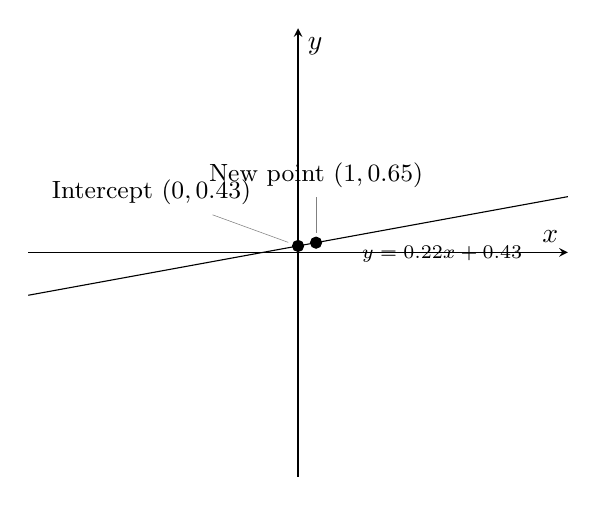
\begin{tikzpicture}
\begin{axis}[
    axis lines=middle,
    xmin=-15, xmax=15,
    ymin=-15, ymax=15,
    xtick=\empty, ytick=\empty,
    xlabel=$x$, ylabel=$y$
]
\addplot[mark=*] coordinates {(0,0.43)} node[pin=140:{\small Intercept $(0,0.43)$}]{} ;
\addplot[mark=*] coordinates {(1,0.65)} node[pin=90:{\small New point $(1,0.65)$}]{} ;
\addplot [domain=-15:15, samples=2] {0.22*x+0.43} node [pos=.6, below right] {\scriptsize $y = 0.22x + 0.43$};
\end{axis}
\end{tikzpicture}
\end{frame}

\myframe{Reading an equation from a graph}
\begin{itemize}
\item Two options:
\begin{enumerate}
\item Slope-intercept form
\begin{enumerate}
\item Find the $y-$intercept
\item Find the slope: how much does $y$ change with each 1 unit difference in $x$?
\end{enumerate}
\item[]
\item Point-slope form
\begin{enumerate}
\item Choose any point on the line
\item Find the slope: how much does $y$ change with each 1 unit difference in $x$?
\end{enumerate}
\end{enumerate}
\end{itemize}

Example: age (years) and height (inches)

Say we have a random sample of 100 pre-school aged-children (age 3--5) from the Seattle area. We expect height to increase with increasing age. We fit the best fitting line to these data to try to better understand these data, and get the plot on the next slide... what are the slope and intercept, and what do they tell us about this association?
\end{frame}

\myframe{Example: reading an equation from a graph}
\centering
\begin{tikzpicture}
\begin{axis}[
    axis lines=middle,
    xmin=-5, xmax=5,
    ymin=0, ymax=50,
    xtick={-5, -4, -3, -2, -1, 0, 1, 2, 3, 4, 5}, 
    ytick={0, 5, 10, 15, 20, 25, 30, 35, 40, 41, 42, 43, 44, 45, 50},
    xlabel=$x$, ylabel=$y$
]
\addplot [domain=-15:15, samples=2] {1.5*x+40} node [pos=.7, below right] {};
\end{axis}
\end{tikzpicture}
\end{frame}

\myframe{Example: reading an equation from a graph}
\centering
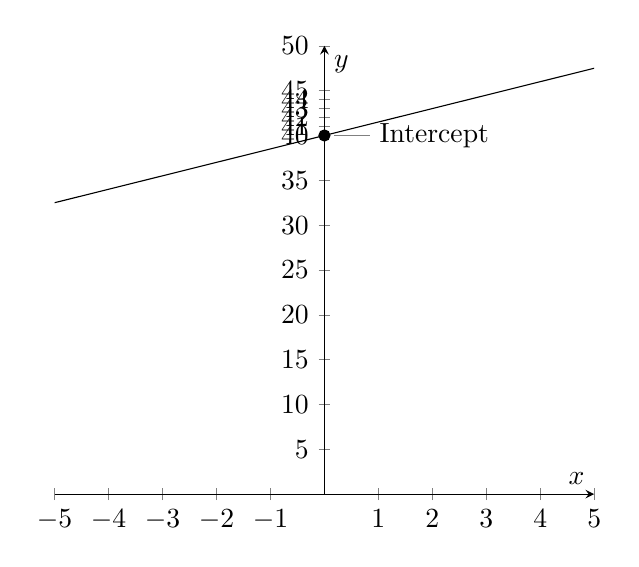
\begin{tikzpicture}
\begin{axis}[
    axis lines=middle,
    xmin=-5, xmax=5,
    ymin=0, ymax=50,
    xtick={-5, -4, -3, -2, -1, 0, 1, 2, 3, 4, 5}, 
    ytick={0, 5, 10, 15, 20, 25, 30, 35, 40, 41, 42, 43, 44, 45, 50},
    xlabel=$x$, ylabel=$y$
]
\addplot [domain=-15:15, samples=2] {1.5*x+40} node [pos=.7, below right] {};
\addplot [mark=*] coordinates {(0,40)} node[pin=0:{Intercept}]{} ;
\end{axis}
\end{tikzpicture}
\end{frame}

\myframe{Example: reading an equation from a graph}
\begin{enumerate}
\item[1.] Find the intercept. Here it is $40$
\end{enumerate}
\centering
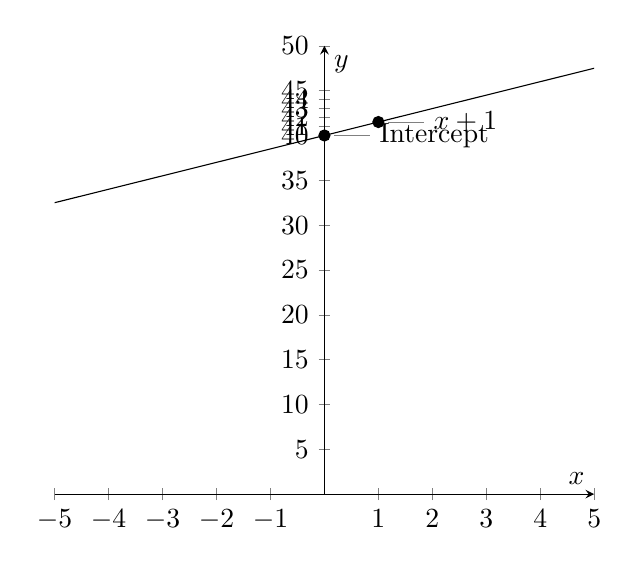
\begin{tikzpicture}
\begin{axis}[
    axis lines=middle,
    xmin=-5, xmax=5,
    ymin=0, ymax=50,
    xtick={-5, -4, -3, -2, -1, 0, 1, 2, 3, 4, 5}, 
    ytick={0, 5, 10, 15, 20, 25, 30, 35, 40, 41, 42, 43, 44, 45, 50},
    xlabel=$x$, ylabel=$y$
]
\addplot [domain=-15:15, samples=2] {1.5*x+40} node [pos=.7, below right] {};
\addplot [mark=*] coordinates {(0,40)} node[pin=0:{Intercept}]{} ;
\addplot [mark=*] coordinates {(1,41.5)} node[pin=0:{$x+1$}]{} ;
\end{axis}
\end{tikzpicture}
\end{frame}

\myframe{Example: reading an equation from a graph}
\begin{enumerate}
\item[2.] Increase $x$ by one to find the slope. The $y$ value at $x = 1$ is $41.5$ (a bit hard to read), so $y$ changed by $1.5$
\end{enumerate}
\centering
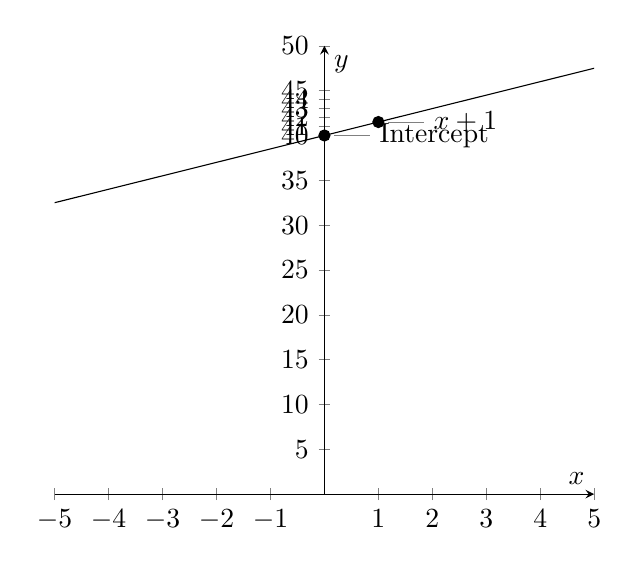
\begin{tikzpicture}
\begin{axis}[
    axis lines=middle,
    xmin=-5, xmax=5,
    ymin=0, ymax=50,
    xtick={-5, -4, -3, -2, -1, 0, 1, 2, 3, 4, 5}, 
    ytick={0, 5, 10, 15, 20, 25, 30, 35, 40, 41, 42, 43, 44, 45, 50},
    xlabel=$x$, ylabel=$y$
]
\addplot [domain=-15:15, samples=2] {1.5*x+40} node [pos=.7, below right] {};
\addplot [mark=*] coordinates {(0,40)} node[pin=0:{Intercept}]{} ;
\addplot [mark=*] coordinates {(1,41.5)} node[pin=0:{$x+1$}]{} ;
\end{axis}
\end{tikzpicture}
\end{frame}

\myframe{Example: reading an equation from a graph}
\begin{enumerate}
\item[3.] Slope-intercept: $y = 1.5x + 40$, point-slope: $y + 40 = 1.5(x-0)$
\end{enumerate}
\centering
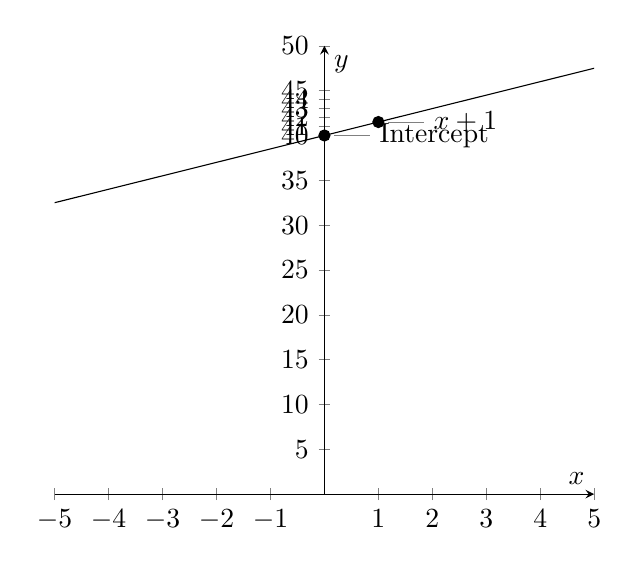
\begin{tikzpicture}
\begin{axis}[
    axis lines=middle,
    xmin=-5, xmax=5,
    ymin=0, ymax=50,
    xtick={-5, -4, -3, -2, -1, 0, 1, 2, 3, 4, 5}, 
    ytick={0, 5, 10, 15, 20, 25, 30, 35, 40, 41, 42, 43, 44, 45, 50},
    xlabel=$x$, ylabel=$y$
]
\addplot [domain=-15:15, samples=2] {1.5*x+40} node [pos=.7, below right] {};
\addplot [mark=*] coordinates {(0,40)} node[pin=0:{Intercept}]{} ;
\addplot [mark=*] coordinates {(1,41.5)} node[pin=0:{$x+1$}]{} ;\end{axis}
\end{tikzpicture}
\end{frame}

\setcounter{subfigure}{0}
\myframe{Exercise: matching graphs to equations}
\begin{enumerate}
\item Which is the graph of $y = 2x - 3$?
\end{enumerate}
\vspace{-2em}
\begin{figure}
\captionsetup[subfigure]{oneside,margin={-3cm,0cm},position=top}
\subfloat[]{
 \resizebox{1.5in}{1.5in}{
  \begin{tikzpicture}
   \begin{axis}[
    axis lines=middle,
    xmin=-5, xmax=5,
    ymin=-5, ymax=5,
    xtick={-5, -4, -3, -2, -1, 0, 1, 2, 3, 4, 5}, 
    ytick={-5, -4, -3, -2, -1, 0, 1, 2, 3, 4, 5},
    xlabel=$x$, ylabel=$y$
   ]
   \addplot [domain=-15:15, samples=2] {1*x-2} node [pos=.7, below right] {};
   \end{axis}
  \end{tikzpicture}
 }
}
\subfloat[]{
\resizebox{1.5in}{1.5in}{
 \begin{tikzpicture}
  \begin{axis}[
    axis lines=middle,
    xmin=-5, xmax=5,
    ymin=-5, ymax=5,
    xtick={-5, -4, -3, -2, -1, 0, 1, 2, 3, 4, 5}, 
    ytick={-5, -4, -3, -2, -1, 0, 1, 2, 3, 4, 5},
    xlabel=$x$, ylabel=$y$
  ]
  \addplot [domain=-15:15, samples=2] {3*x-3} node [pos=.7, below right] {};
  \end{axis}
 \end{tikzpicture}
 }
}
\vspace{-2em}
\subfloat[]{
\resizebox{1.5in}{1.5in}{
 \begin{tikzpicture}
  \begin{axis}[
    axis lines=middle,
    xmin=-5, xmax=5,
    ymin=-5, ymax=5,
    xtick={-5, -4, -3, -2, -1, 0, 1, 2, 3, 4, 5}, 
    ytick={-5, -4, -3, -2, -1, 0, 1, 2, 3, 4, 5},
    xlabel=$x$, ylabel=$y$
  ]
  \addplot [domain=-15:15, samples=2] {.5*x+1} node [pos=.7, below right] {};
  \end{axis}
 \end{tikzpicture}
 }
}
\subfloat[]{
\resizebox{1.5in}{1.5in}{
 \begin{tikzpicture}
  \begin{axis}[
    axis lines=middle,
    xmin=-5, xmax=5,
    ymin=-5, ymax=5,
    xtick={-5, -4, -3, -2, -1, 0, 1, 2, 3, 4, 5}, 
    ytick={-5, -4, -3, -2, -1, 0, 1, 2, 3, 4, 5},
    xlabel=$x$, ylabel=$y$
  ]
  \addplot [domain=-15:15, samples=2] {2*x-3} node [pos=.7, below right] {};
  \end{axis}
 \end{tikzpicture}
 }
}
\end{figure}
\end{frame}

\myframe{Solution: matching graphs to equations}
\begin{itemize}
\item[(a)] Intercept: $-2$, slope: 1
\item[]
\item[(b)] Intercept: $-3$, slope: 3
\item[]
\item[(c)] Intercept: $1$, slope: 1
\item[]
\item[(d)] Intercept: $-3$, slope: 2 \checkmark
\end{itemize}
\end{frame}

\section{Quadratics}
\myframe{Quadratics}
\begin{itemize}
\item Sometimes we believe a trend is higher order than linear
\begin{itemize}
\item For example, height might increase more quickly with age at a younger age, and then level off at older ages
\end{itemize}
\item[]
\item Higher order terms allow more flexibility in modeling
\item[]
\item Quadratics are the natural next step from linear terms, and are shaped like parabolas
\end{itemize}
\end{frame}

\myframe{Defining a quadratic}
\begin{itemize}
\item Standard form: $y = ax^2 + bx + c$
\item[]
\item $a$ determines the direction of the tails and the degree of curvature
\begin{itemize}
\item $a > 0$ means the curve faces up (convex)
\item $a < 0$ means the curve faces down (concave)
\item large $|a| > 1$ means steep slope
\item $0 < |a| < 1$ means shallow slope
\end{itemize}
\item[]
\item $b$ and $a$ together determine the $x-$coordinate of the vertex: $x = -\frac{b}{2a}$
\item[]
\item $c$ controls the height
\end{itemize}
\end{frame}

\myframe{Example: quadratics}
\begin{itemize}
\item $y = x^2 + 2$
\item[]
\item $a = 1$, $b = 0$, $c = 2$
\item[]
\item Not too steep, convex, and vertex is at $(0, 2)$
\end{itemize}
\centering
\begin{tikzpicture}
  \begin{axis}[
    axis lines=middle,
    xmin=-5, xmax=5,
    ymin=-5, ymax=5,
    xtick={-5, -4, -3, -2, -1, 0, 1, 2, 3, 4, 5}, 
    ytick={-5, -4, -3, -2, -1, 0, 1, 2, 3, 4, 5},
    xlabel=$x$, ylabel=$y$
  ]
  \addplot [domain=-15:15, samples=100] {x^2+2} node [pos=.7, below right] {};
  \end{axis}
 \end{tikzpicture}
\end{frame}

\myframe{Example: quadratics}
\begin{itemize}
\item $y = -2x^2 + 3x + 2$
\item[]
\item $a = -2$, $b = 3$, $c = 2$
\item[]
\item Steeper than before, concave, and vertex is at $(3/4, 50/16)$
\end{itemize}
\centering
\begin{tikzpicture}
  \begin{axis}[
    axis lines=middle,
    xmin=-5, xmax=5,
    ymin=-5, ymax=5,
    xtick={-5, -4, -3, -2, -1, 0, 1, 2, 3, 4, 5}, 
    ytick={-5, -4, -3, -2, -1, 0, 1, 2, 3, 4, 5},
    xlabel=$x$, ylabel=$y$
  ]
  \addplot [domain=-15:15, samples=100] {-2*x^2+3*x+2} node [pos=.7, below right] {};
  \end{axis}
 \end{tikzpicture}
\end{frame}


\setcounter{subfigure}{0}
\myframe{Exercise: quadratics}
\begin{enumerate}
\item Which is a plausible plot of $x^2 - x + 2$?
\end{enumerate}
\vspace{-2em}
\begin{figure}
\captionsetup[subfigure]{oneside,margin={-3cm,0cm},position=top}
\subfloat[]{
 \resizebox{1.5in}{1.5in}{
  \begin{tikzpicture}
   \begin{axis}[
    axis lines=middle,
    xmin=-5, xmax=5,
    ymin=-5, ymax=5,
    xtick={-5, -4, -3, -2, -1, 0, 1, 2, 3, 4, 5}, 
    ytick={-5, -4, -3, -2, -1, 0, 1, 2, 3, 4, 5},
    xlabel=$x$, ylabel=$y$
   ]
   \addplot [domain=-15:15, samples=100] {x^2-x+2} node [pos=.7, below right] {};
   \end{axis}
  \end{tikzpicture}
 }
}
\subfloat[]{
\resizebox{1.5in}{1.5in}{
 \begin{tikzpicture}
  \begin{axis}[
    axis lines=middle,
    xmin=-5, xmax=5,
    ymin=-5, ymax=5,
    xtick={-5, -4, -3, -2, -1, 0, 1, 2, 3, 4, 5}, 
    ytick={-5, -4, -3, -2, -1, 0, 1, 2, 3, 4, 5},
    xlabel=$x$, ylabel=$y$
  ]
  \addplot [domain=-15:15, samples=100] {x^2-2*x+2} node [pos=.7, below right] {};
  \end{axis}
 \end{tikzpicture}
 }
}
\vspace{-2em}
\subfloat[]{
\resizebox{1.5in}{1.5in}{
 \begin{tikzpicture}
  \begin{axis}[
    axis lines=middle,
    xmin=-5, xmax=5,
    ymin=-5, ymax=5,
    xtick={-5, -4, -3, -2, -1, 0, 1, 2, 3, 4, 5}, 
    ytick={-5, -4, -3, -2, -1, 0, 1, 2, 3, 4, 5},
    xlabel=$x$, ylabel=$y$
  ]
  \addplot [domain=-15:15, samples=100] {x^2-x-2} node [pos=.7, below right] {};
  \end{axis}
 \end{tikzpicture}
 }
}
\subfloat[]{
\resizebox{1.5in}{1.5in}{
 \begin{tikzpicture}
  \begin{axis}[
    axis lines=middle,
    xmin=-5, xmax=5,
    ymin=-5, ymax=5,
    xtick={-5, -4, -3, -2, -1, 0, 1, 2, 3, 4, 5}, 
    ytick={-5, -4, -3, -2, -1, 0, 1, 2, 3, 4, 5},
    xlabel=$x$, ylabel=$y$
  ]
  \addplot [domain=-15:15, samples=100] {-x^2-x+2} node [pos=.7, below right] {};
  \end{axis}
 \end{tikzpicture}
 }
}
\end{figure}
\end{frame}

\myframe{Solution: quadratics}
\begin{enumerate}
\item $a = 1$, $b = -1$, $c = 2$
\begin{itemize}
\item We are looking for a plot where the vertex has $y-$coordinate near 2
\item[]
\item This rules out (b)
\item[]
\item Now we want a plot with $y = 2$ when $x = 1$, ruling out (b) [and (d)]
\item[]
\item Of the two remaining, (d) is concave, so it has $a < 0$
\item[]
\item (a) is the solution!
\end{itemize}
\end{enumerate}
\end{frame}

\section{Transformations}
\myframe{Transforming graphs}
In the example of the association between FEV and age, we obtained the line $y = 0.22x + 0.43$; this means that \textcolor{red}{children at age 0 have a mean FEV of 0.43 L/sec}, and that \textcolor{blue}{mean FEV tends to be 0.22 L/sec higher for each one year increase in age}.

How can we make the \textcolor{red}{intercept} interpretable? What would the association be if the slope were different, and what would this look like? What would happen if we changed the units on FEV (to, say, mL/sec)? 

These are all examples of \textcolor{green}{transformations}:
\begin{itemize}
\item Once we have one graph, how do we get another?
\item[]
\item Two main types of transformations: shifting and stretching
\end{itemize}
\end{frame}

\myframe{Shifting graphs}
\begin{itemize}
\item Sometimes we want to change the interpretation of the intercept
\begin{itemize}
\item FEV data: e.g., we could make the intercept the mean FEV at the \textcolor{blue}{average age} in the data
\end{itemize}
\item[]
\item Once we know the properties of a graph, shifting doesn't change much!
\item[]
\item Shift left: add to $x$
\item[]
\item Shift right: subtract from $x$
\item[]
\item Shift up: add to intercept
\item[]
\item Shift down: subtract from intercept
\item[]
\item Why? Adding to $x$: smaller $x$'s now have the same $y$. Subtracting from $x$: larger $x$'s now have the same $y$.
\end{itemize}
\end{frame}

\myframe{Example: shifting graphs}
{\centering
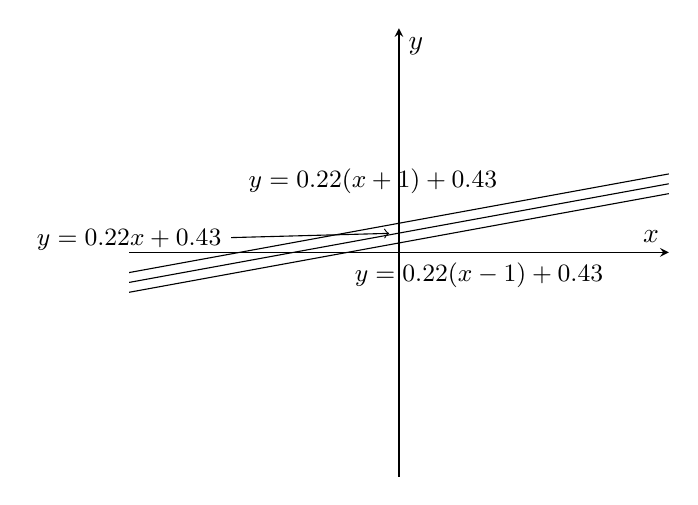
\begin{tikzpicture}
  \begin{axis}[
    axis lines=middle,
    xmin=-5, xmax=5,
    ymin=-5, ymax=5,
    xtick=\empty, 
    ytick=\empty,
    xlabel=$x$, ylabel=$y$
  ]
  \addplot [domain=-5:5, samples=2] {0.22*(x+1) + 0.43} node [pos=.7, above left] {\small $y = 0.22(x+1) + 0.43$};
  \addplot [domain=-5:5, samples=2] {0.22*x + 0.43} node (a) [pos=.5] {};
  \addplot [domain=-5:5, samples=2] {0.22*(x-1) + 0.43} node [pos=.4, below right] {\small $y = 0.22(x-1) + 0.43$};
  \end{axis}
  \node[draw=none] (b) at (0,3) {\small $y = 0.22x + 0.43$}; 
  \draw [->] (b) -- (a); 
 \end{tikzpicture}
}

\scriptsize
Interpretations (from top to bottom): 
\begin{spaceitemize}
\item mean FEV in $-1$ year olds is 0.21 L/sec
\item mean FEV in zero year olds is 0.43 L/sec
\item mean FEV in one year olds is 0.65 L/sec
\end{spaceitemize} 
\end{frame}

\myframe{Stretching graphs}
If we change the units on our predictor of interest, we will change the slope (and hence the interpretation). We also might want to see how the graph would change if the slope were larger or smaller, using the same units---this helps to understand the estimated association between our predictor and the outcome.

These are examples of \textcolor{green}{stretching}:
\begin{itemize}
\item Make the graph steeper, or shrink it: make $|m|$ larger in a linear equation, and make $|a|$ larger in a quadratic equation
\item[]
\item Make the graph shallower, or stretch it: make $|m|$ smaller in a linear equation, and make $|a|$ smaller in a quadratic equation
\end{itemize}
\end{frame}

\myframe{Example: stretching graphs}
\centering
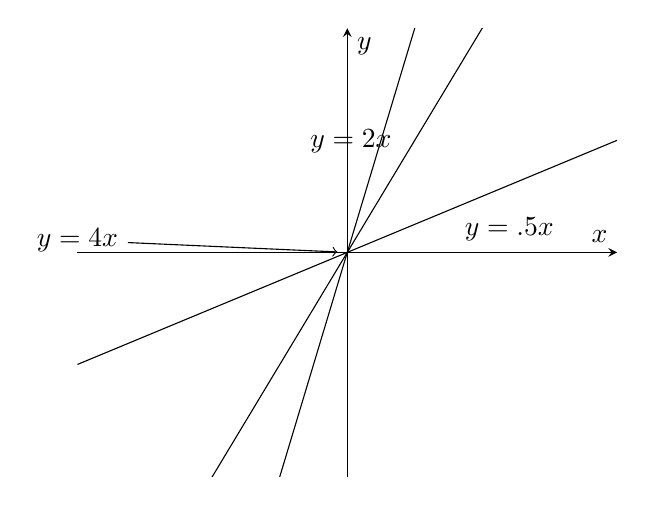
\begin{tikzpicture}
  \begin{axis}[
    axis lines=middle,
    xmin=-5, xmax=5,
    ymin=-5, ymax=5,
    xtick=\empty, 
    ytick=\empty,
    xlabel=$x$, ylabel=$y$
  ]
  \addplot [domain=-5:5, samples=2] {2*x} node [pos=.6, above left] {$y = 2x$};
  \addplot [domain=-5:5, samples=2] {4*x} node (a) [pos=.5] {};
  \addplot [domain=-5:5, samples=2] {.5*x} node [pos=.7, below right] {$y = .5x$};
  \end{axis}
  \node[draw=none] (b) at (0,3) {$y = 4x$}; 
  \draw [->] (b) -- (a); 
 \end{tikzpicture}
\end{frame}

\myframe{Exercise: transforming graphs}
\begin{enumerate}
\item How do we shift the graph of $y = 2x + 3$ one unit right?
\item[]
\item How do we transform the graph of $y = 2x + 3$ to have a shallower slope?
\item[]
\item How do we transform the graph of $y = 2x + 3$ to have a slope of $1$ and a $y-$intercept of 4?
\end{enumerate}
\end{frame}

\myframe{Solution: shifting graphs}
\begin{enumerate}
\item Subtract 1 from $x$! New equation: $y = 2(x-1) + 3$
\item[]
\item Multiply by a number less than $1$; for example, take $x/2$. This gives new equation $y = 2(x/2) + 3$, or $y = x + 3$
\item[]
\item To get a slope of 1, divide $x$ by 2. To make the $y-$intercept 4, shift left by adding $1/2$ to $x$. New equation: $y = 2*(x/2 + 1/2) + 3$, or $y = x + 4$
\end{enumerate}
\end{frame}

\myframe{Summary}
\begin{itemize}
\item Graphs are useful tools to describe relationships in data or visualize functions
\item[]
\item Histograms, boxplots, and scatterplots are common and useful types of graphs
\item[]
\item Linear trends can be described in:
\begin{itemize}
\item Slope-intercept form --- $y = mx + b$
\item Point-slope form --- $y - y_1 = m(x - x_1)$
\end{itemize}
\item[]
\item Reading an equation from a graph involves finding the intercept and calculating the slope
\item[]
\item Graphs can be transformed by adding/subtracting from $x$, or multiplying/dividing $x$
\end{itemize}
\end{frame}
\end{document}
